This Section introduces the concept of data mananagement layer, starting from its origin and evolution in to today's technologies. This dissertation includes advantages and limitations of each evolutive step, and describe the functions of \gls{DBMS}. what a data storage is and which typologies of storages exist. The Subsections \ref{subsec:datalakehouse_architecture} focuses on the architecture of data lakehouses, explaing in details each component involed. Then, in Subsections \ref{subsec:datalakehouse_comparison}, three data lakehouse frameworks are compared, namely Hudi, employed in the legacy version of Hopsworks feature store, Iceberg and Delta Lake, the two alternatives evaluated.

\subsection{Brief history of \glsfmtlongpl{DBMS}}
\label{subsec:history_DBMS}
Since the 2010s, with the advent of Big Data, the data volume, variety, and production velocity have increased exponentially \cite{ederUnstructuredData802008, penceWhatBigData2014}. While on one side, this proved to be of enormous value, on the other this posed several challenges \cite{demchenkoAddressingBigData2012} on data architectures, which had to evolve to cope with these new needs. Data lakehouse frameworks, like Hudi, Iceberg and Delta Lake \cite{rajaperumalUberEngineeringIncremental2017,IcebergExamples2024,armbrustDeltaLakeHighperformance2020} are the last step of this evolution. However, to truly understand this tools, it is needed to start from the beginning of \gls{DBMS} evolution.

\smallskip

Before big data, companies already wanted to get insights from their data, automating the workflow from the data sources to point of access to this dataa. Here is where \gls{ETL} and relational databases first came into use. An \gls{ETL} pipeline consists of three steps:
\begin{enumerate}
    \item \textbf{Extracts} data from \glspl{API} or other various data sources.
    \item \textbf{Transforms} data according to one or more goal. Often this means removing absent fields, standardizes to a specific format to match the database schema, and validates the data.
    \item \textbf{Loads} it into a relational database (e.g., MySQL).
\end{enumerate}
This workflow structure enabled companies to generate \gls{BI} insights and data reports based on organizational data. However, a key limitation of this approach is its restricted ability to perform analytical queries that require joining multiple tables and working on several data dimensions. These types of queries, while executed less frequently than simpler queries, are essential for strategic decision-making (e.g., identifying the customer segment with the highest profitability over the past year, with the capabilities of drilling down on products, marketing and sales information).

\smallskip

To address the increasing demand for analytical queries, more advanced \glspl{DBMS} replaced traditional relational databases, optimizing performance for business-oriented analytical workloads. These systems, known as \glspl{OLAP}, introduced specialized storage and query execution strategies tailored for large-scale analytical processing. The most notable example of an \gls{OLAP} system is the data warehouse, which revolutionized how organizations handle structured data analysis. A data warehouse workflow, enables companies to process and analyze significantly larger datasets than traditional databases. Unlike transactional databases, which optimize for rapid insert/update operations, data warehouses focus on read-optimized queries by structuring data into columnar formats, reducing scan times for analytical queries. They maintain core relational database properties such as \gls{ACID} transactions and data versioning, ensuring data integrity and consistency for complex business intelligence applications.  

\smallskip

Over time, the exponential growth of unstructured data (e.g., images, videos, logs, and sensor data), posed new challenges for companies aiming to leverage such information. Traditional data warehouses struggled to accommodate this data due to their rigid schema requirements and high storage costs. Moreover, they were not designed to support \gls{AI}/\gls{ML} workflows that rely on diverse, unstructured datasets. To overcome these limitations, organizations adopted a new paradigm known as data lakes. Data lakes leverage cost-efficient object storage (Section~\ref{subsec:block_vs_file_vs_object}) and a schema-on-read approach, where raw data is loaded first and transformed only when needed. This shift from the traditional \gls{ETL} model to \gls{ELT} offers greater flexibility in handling diverse data types. For example, businesses can use data lakes to store raw IoT sensor readings and later refine them for predictive maintenance models, once the needed data transformation will be designed. Despite reducing storage costs and improving flexibility, data lakes introduced new complexities. Unlike structured databases, querying data lakes directly for \gls{BI} reports is impractical, as they lack indexing and transactional consistency. Additionally, maintaining separate storage solutions for structured (data warehouses) and unstructured (data lakes) data increases operational complexity and costs. A major drawback of data lakes is the risk of becoming "data swamps", repositories filled with ungoverned, low-quality data that provide little business value. Recognizing these challenges, organizations sought a hybrid solution combining the best features of data warehouses and data lakes. This led to the emergence of the data lakehouse architecture. First described by Databricks in 2020 at \gls{CIDR} \cite{lakehouse2021}, data lakehouses integrate structured and unstructured data storage capabilities of data lakes, while maintaining the governance, \gls{ACID} compliance, and indexing capabilities of data warehouses. The data lakehouse approach resolves many pain points associated with separate data warehouses and data lakes. It enables organizations to use a single storage for all types of data, while supporting high-performance \gls{SQL} queries and \gls{ML} workloads. Furthermore, by leveraging open file formats like Apache Parquet, ORC and Avro, data lakehouses ensure interoperability with various analytics engines, avoiding the risk of getting data locked into a proprietary format \cite{mazumdarDataLakehouseData2023}. All these capabilities and features make lakehouses an ideal solution for enterprise-scale data processing. Table \ref{tab:DBMS_comparison} provides a comparison of data warehouses, data lakes, and data lakehouses, highlighting key takeaways for each technology and summarizing what described so far.

\begin{table}[!h]
    \centering
    \caption[Comparison of data architectures]{Comparison of key features of Data Warehouses, Data Lakes, and Data Lakehouses \cite{inmonFiveStepsSuccessful}.}
    \label{tab:DBMS_comparison}
    \begin{tabular}{|p{2.2cm}|p{3cm}|p{2.9cm}|p{3cm}|}
        \hline
        \textit{\textbf{Feature}} & \textbf{Data Warehouse} & \textbf{Data Lake} & \textbf{Data Lakehouse} \\
        \hline
        \textit{Primary Use} & Business Intelligence, \gls{SQL} Analytics & Unstructured data storage, \gls{AI}/\gls{ML} workflows & Unified storage for structured/unstructured data, \gls{SQL} + \gls{AI}/\gls{ML} processing \\
        \hline
        \textit{Data Type} & Structured & Unstructured & All data types \\
        \hline
        \textit{Query Performance} & Optimized for \gls{SQL}-based queries, fast indexed access & Slow for structured queries, requires extensive data preparation & High performance for both \gls{SQL} and \gls{ML} workloads \\
        \hline
        \textit{Schema Enforcement} & Strict schema-on-write & Schema-on-read & Flexible schema with enforcement and evolution support \\
        \hline
        \textit{\gls{ACID} support} & Fully supported & Not supported & Fully supported \\
        \hline
        \textit{Scalability} & Limited scalability due to high storage costs & High scalability, low-cost storage & Highly scalable with structured query optimizations \\
        \hline
        \textit{Storage Cost} & High due to proprietary formats & Low due to object storage & Moderate, optimized for efficiency \\
        \hline
        \textit{Governance} & Strong governance, access control, and security & Weak governance, risk of data swamps & Fine-grained governance with access control and security \\
        \hline
        \textit{Key Takeaways} & Best for structured data and BI queries. High-performance \gls{SQL} analytics. & Ideal for cost-effective big data storage. Difficult to manage and query efficiently & Combines the best of warehouses and lakes. Supports both \gls{SQL} and \gls{AI}/\gls{ML} use cases efficiently. \\
        \hline
    \end{tabular}
\end{table}



\subsection{Data lakehouse architecture}
\label{subsec:datalakehouse_architecture}
Data lakehouse architectures combines the desirable attributes of data warehouses and data lakes, mitigating the challenges encountered by both these technologies, and eliminate the need of a two-tier data stacks to run varying analytical workloads. The key components of data lakehouses are at the bases of any other architecture seen so far, but their design focus on reducing components coupling, providing more agility and choice when architecting such platform \cite{mazumdarDataLakehouseData2023}. The data lakehouse components, graphically presented in Figure \ref{fig:lakehouse_schema}, are:

\begin{itemize}
    \item \textbf{Data storage}: is where data files land after ingestion from various systems, usually a Cloud object store, as described in Section \ref{sec:back_data_storage}.
    \item \textbf{File formats}: hold the actual raw data and are phisically stored in the data storage. They are open-source file formats, such Apache Parquet or JSON, and are typically column-oriented.
    \item \textbf{Table format}: also referred as \gls{OTF}, acts as metadata layer on the top of the file formats, that abstracts the underlying physical data structure. They offers \gls{API} access to the query and storage engines.
    \item \textbf{Storage engine}: handles data management tasks, aimed at optimizing efficiency of queries over the data. It performes tasks as data compation, indexing, and partitioning.
    \item \textbf{Catalog}: sometimes described as metastore, it enables efficient search and discovery. The catalog keeps track of information about each table (name, column names, data types) and a reference to metadata for each table (table format).
    \item \textbf{Query engine}: is responsible for processing data, performing read and write operarations leveraging the table format \gls{API}. They are further explained in Section \ref{sec:back_query_engine}.
\end{itemize}

\begin{figure}[!ht]
    \begin{center}
      \includegraphics[width=0.6\textwidth]{figures/2-background_and_related_work/lakehouse_schema.png}
    \end{center}
    \caption[Architecture of data lakehouse]{Abstraction of architecture of a data lakehouse. Inspired by "Open table formats in perspective" article on OneHouse Website, available at \url{https://www.onehouse.ai/blog/open-table-formats-and-the-open-data-lakehouse-in-perspective}}
    \label{fig:lakehouse_schema}
\end{figure}

\gls{OTF} are open standards, and by design support interoperability throughout the stack, as visible in Figure \ref{fig:lakehouse_schema}. Thus, depending on the integration capabilities of the table format, there are several implementation options for data storage, file formats, storage engine, catalog and query engine. Additionally, recent introduction of tools like Apache XTable~\footnote{XTable repository available at \url{https://xtable.apache.org/}} demonstrates the trend towards a universal compatibility between \glspl{OTF}.


\subsubsection*{Open Table Formats}

\glspl{OTF} provide an abstraction layer on top of data lakes, enabling database-like functionalities, enhancing data management capabilities significantly \cite{lakehouse2021,DataLakehouseSurvey2025}. One of the cornerstone features of \glspl{OTF} is support for full \gls{CRUD} operations. The ability to perform updates and deletes sets datalake house data storage apart from traditional file-based storages, where such operations are cumbersome and inefficient. Performance and scalability are other notable features that \glspl{OTF} bring to the table. These formats are designed to excel in Big Data environments, where data volumes are massive and continue to grow. \glspl{OTF} could support various optimization techniques, such as indexing, partitioning, and caching, to expedite data retrieval and processing. This not only improves query performance but also ensures that the system can scale horizontally to accommodate increasing data loads without a significant degradation in performance. As a result, organizations can manage their data ecosystems more effectively, making data-driven insights more accessible and actionable. Transactional support with \gls{ACID} compliance is another key feature of \glspl{OTF}. This ensures that all data transactions are processed reliably, maintaining data integrity and consistency across the board. This is particularly important in scenarios where multiple transactions occur simultaneously or when the system needs to recover from partial failures. \glspl{OTF} guarantee that each transaction is completed successfully or fully rolled back, providing an essential level of data reliability and trustworthiness for critical business operations. This comprehensive functionality allows for flexible and complex data workflows, and ensures that data lakes and warehouses can be updated in real time, reflecting the most current state of information.



\subsection{Data lakehouse comparison}
\label{subsec:datalakehouse_comparison}

The three main data lakehouse frameworks investigated in this project are Hudi \cite{rajaperumalUberEngineeringIncremental2017}, Iceberg \cite{IcebergExamples2024} and Delta Lake \cite{armbrustDeltaLakeHighperformance2020}. Their popularity has increased proportionally with the popularity of the data lakehouse architecture, as visible by the growing community of each of these technologies in Figure \ref{fig:github_stars}, becoming the de-facto standards for data lakehouse implementations \cite{jainAnalyzingComparingLakehouse2023}. Some alternatives are newly being developed, such Apache Paimon~\footnote{GitHub repository available at \url{https://github.com/apache/paimon/}.}, but are still at early stages of their development and will not investigated in this thesis project. The following subsections present each of these technologies, specifying their development history, key features, integration capabilities, \gls{API} offered and in which are the use cases they are most suitable for. \todo{Maybe add some schema about the metadata layer for each technology.}

\begin{figure}[h]
    \centering
    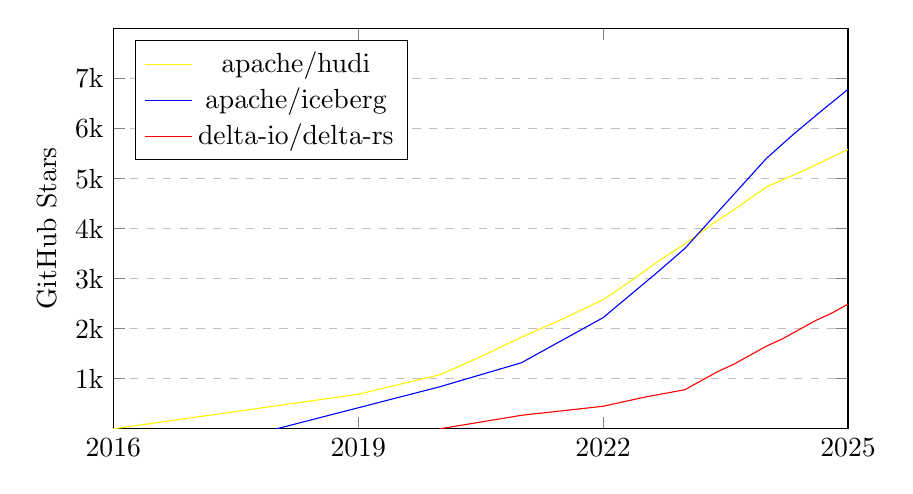
\begin{tikzpicture}
        \begin{axis}[
            ylabel={GitHub Stars},
            xmin=2016, xmax=2025,
            ymin=0, ymax=8000,
            xtick={2016, 2019, 2022, 2025},
            xticklabels={2016, 2019, 2022, 2025},
            ytick={1000, 2000, 3000, 4000, 5000, 6000, 7000},
            yticklabels={1k, 2k, 3k, 4k, 5k, 6k, 7k},
            legend pos=north west,
            ymajorgrids=true,
            grid style=dashed,
            width=0.9\textwidth,
            height=0.55\textwidth,
        ] 
        \addplot[color=yellow] coordinates {
            (2016, 0)
            (2019, 690)
            (2020, 1080)
            (2020.5, 1440)
            (2021, 1830)
            (2021.5, 2190)
            (2022, 2580)
            (2022.33, 2940)
            (2022.66, 3330)
            (2023, 3690)
            (2023.33, 4080)
            (2023.66, 4440)
            (2024, 4830)
            (2024.5, 5190)
            (2025, 5580)
        };
        \addlegendentry{apache/hudi}
        \addplot[color=blue] coordinates {
            (2018, 0)
            (2020, 840)
            (2021, 1320)
            (2021.5, 1770)
            (2022, 2220)
            (2022.33, 2670)
            (2022.66, 3120)
            (2023, 3600)
            (2023.25, 4050)
            (2023.50, 4500)
            (2023.75, 4950)
            (2024, 5400)
            (2024.33, 5880)
            (2024.66, 6330)
            (2025, 6780)
        };
        \addlegendentry{apache/iceberg}
        \addplot[color=red] coordinates {
            (2020, 0)
            (2021, 270)
            (2022, 450)
            (2022.5, 630)
            (2023, 780)
            (2023.2, 960)
            (2023.4, 1140)
            (2023.6, 1290)
            (2023.8, 1470)
            (2024, 1650)
            (2024.2, 1800)
            (2024.4, 1980)
            (2024.6, 2160)
            (2024.8, 2310)
            (2025, 2490)
        };
        \addlegendentry{delta-io/delta-rs}
        \end{axis}
    \end{tikzpicture}
    \caption[GitHub stars of \glspl{OTF} repositories]{Trend of GitHub stars of following repositories \url{https://github.com/apache/iceberg}, \url{https://github.com/apache/hudi}, \url{https://github.com/delta-io/delta-rs}.}
    \label{fig:github_stars}
\end{figure}

\subsubsection*{Apache Hudi}
Apache Hudi, open-sourced by Uber in 2017 \cite{rajaperumalUberEngineeringIncremental2017}, is an open-source framework that addresses the challenges of low-latency data ingestion and incremental processing. Hudi enables efficient record updates and deletions in data lakes, thus eliminating the need to rewrite entire datasets \cite{hudi_tech_docs}. The framework supports \gls{CDC} for efficient updates and deletes. Hudi offers two primary write optimization modes: \gls{CoW} for high read performance and \gls{MoR} for balancing both write and read performance. 

Hudi's metadata layer is structured around a timeline-based architecture, maintaining a history of all table operations, thus providing version control. The commit timeline records actions such as inserts, updates, deletes, and compactions, enabling time travel by referencing specific commit instants. The metadata table optimizes file listing by indexing data files, partitions, and record locations, improving query performance. Hudi also maintains delta logs (\gls{MoR}) to track incremental changes before they are compacted into columnar storage. The file groups and file slices structure organizes base and log files, ensuring efficient data versioning. 

Hudi is optimized for real-time analytics through low-latency streaming ingestion, and integrates seamlessly with Spark and Flink for data ingestion and processing. Hudi also supports reading data from Hive, Impala, and Presto. The framework incorporates multimodal indexing, such as Bloom filters and record-level indexing, and employs both Multi-Version \gls{CC} and Optimistic \gls{CC} for transaction management. Typical use cases for Hudi include streaming ingestion with frequent updates and deletes, incremental data processing, and real-time updates in domains like IoT, fintech, and log data processing \cite{comparison1_LakeFS}. While Hudi excels in real-time ingestion, its metadata overhead can be significant for large-scale analytical queries, potentially resulting in slower query performance compared to other formats like Iceberg and Delta Lake \cite{comparison4_starburst}.

Hudi's core implementation is in Java, and it integrates deeply with Apache Spark, offering a Spark datasource \gls{API} for reading and writing Hudi tables.  This makes Java and Scala the primary languages for Hudi development and usage.  While a standalone Python \gls{SDK} for Hudi doesn't exist, Python users can still interact with Hudi tables through PySpark, leveraging the Spark \gls{API}.  Although community-driven efforts like hudi-rs~\footnote{hudi-rs repository available at \url{https://github.com/apache/hudi-rs}.}, a native Rust implementation with Python bindings, are emerging, offering read support for some technologies, Hudi is currently still \gls{JVM}-centric.



\subsubsection*{Apache Iceberg}
Apache Iceberg, open-sourced by Netflix in 2018 \cite{IcebergExamples2024}, is an open-source framework that addresses the limitations of Hive tables by emphasizing scalability and correctness for large-scale analytics. By separating metadata from data, Iceberg supports efficient snapshot-based isolation and query planning \cite{shiranApacheIcebergDefinitive2024,iceberg_tech_docs}. The framework provides full \gls{ACID} transactions, ensuring atomicity, consistency, isolation, and durability. Iceberg allows for schema evolution, enabling the addition, removal, and renaming of columns, without breaking existing queries. It also supports partition evolution, allowing changes to partitioning schemes without necessitating data rewrites. 

Iceberg's metadata layer consists of multiple components that enable efficient time travel and point-in-time query planning. The manifest list acts as an index, pointing to multiple manifest files, each of which tracks a subset of data files. These manifest files store information about data file locations, partitioning, and statistics (e.g., min/max values). The snapshot metadata records changes over time, referencing manifest lists and enabling time travel by tracking table versions. Iceberg also maintains a table metadata file, which holds high-level properties, schema, partitioning details, and references to the latest snapshot. 

Iceberg is designed to scale to petabyte-scale datasets with optimized metadata management using manifest files. Its architecture enables data warehouse-like functionality, leveraging cloud object storage for efficient data access. Furthermore, Iceberg supports collaboration across multiple applications with transactionally consistent access. The framework integrates with query engines like Spark, Trino, Presto, and Dremio and supports Flink for both reading and writing. Iceberg excels in read performance, particularly for tables with large numbers of partitions \cite{comparison1_LakeFS}. It is ideal for analytical workloads that involve large-scale datasets and frequent schema or partition evolution. However, Iceberg's write performance may not be as optimized for streaming scenarios compared to other formats.

Iceberg's core is written in Java, and it is heavily integrated with Apache Spark \cite{IcebergNewHadoop,iceberg_tech_docs}.  The most common way to interact with Iceberg is through SparkSQL or other query engines like Trino and Presto, which support Iceberg natively, making Java and Scala the dominant languages in these environments.  However, Iceberg offers more than just Spark bindings. PyIceberg \cite{PyIceberg} provides a direct Python interface for read and -- from release 0.6.0 in 2024 -- write operations, making Iceberg accessible to Python developers without requiring PySpark.  Furthermore, query engines like Trino, accessible from Python via libraries like PyHive, allow Python users to query Iceberg tables through \gls{SQL}. Iceberg community has recently developed a Rust implementation, iceberg-rust~\footnote{iceberg-rust available at \url{https://github.com/apache/iceberg-rust}.}, which provides read access to Iceberg tables, further expanding its accessibility to a wider range of language ecosystems.



\subsubsection*{Delta Lake}
Delta Lake, open-sourced by Databricks in 2019 \cite{armbrustDeltaLakeHighperformance2020}, is an open-source framework that enhances the reliability and performance of data lakes, facilitating a seamless transition between batch and streaming use cases. Often considered the first data lakehouse, Delta Lake employs a transaction log to record all changes to data, ensuring consistent views and write isolation, which supports concurrent data operations \cite{deltalake_tech_docs}. The framework offers \gls{ACID} transactions, as well as features such as unified batch and streaming processing, indexing, and schema enforcement.

Delta Lake's metadata layer is built around the Delta Log, which records every transaction in JSON files, enabling time travel. The transaction log maintains a sequential history of operations, while checkpoint files (stored in Parquet format) periodically summarize log entries for faster metadata access. The protocol metadata defines the table's versioning, schema, and supported features, ensuring compatibility across different readers and writers. It also incorporates metadata-informed data skipping during merge operations and supports streaming through change data feeds.

Delta Lake tighlty integrates with Spark, thus it is particularly well-suited for real-time streaming, batch processing, and \gls{ML} pipelines requiring data versioning. While its open-source adoption continues to grow, Delta Lake remains deeply integrated with the Databricks ecosystem \cite{jainAnalyzingComparingLakehouse2023,comparison2_medium_recent}. Additionally, its focus on schema and partition evolution is less pronounced compared to frameworks like Iceberg, making Delta Lake less suitable for situations where data schemas are frequently changing.

Delta Lake  core is written in Java and Scala \cite{deltalake_tech_docs}, providing native support within the Spark ecosystem through the delta package. This allows Java and Scala developers to interact directly with Delta tables. Python support is provided via PySpark, enabling Python developers to leverage the Spark \gls{API} for Delta Lake operations.  However, Delta Lake's reach extends beyond the \gls{JVM}.  With the release of Delta Kernel \cite{AnnouncingDeltaLake2023}, a Java library providing low-level access, and the development of delta-rs~\footnote{delta-rs repository available at \url{https://github.com/delta-io/delta-rs}.}, a Rust-based implementation, Delta Lake has become accessible to a wider audience.  The library delta-rs allows interaction with Delta tables without Spark or \gls{JVM} dependencies, and its Python bindings makes this particularly attractive to the Python data science community.



\medspace
In Table \ref{table:lakehouse_comparison} is presented a comparation between key features of the three data lakehouse frameworks.



\begin{table}[!h]
    \centering
    \caption[Comparison of data lakehouses]{Comparison of key features of Apache Hudi, Apache Iceberg, Delta Lake \cite{hudi_tech_docs,iceberg_tech_docs,deltalake_tech_docs}.}
    \label{table:lakehouse_comparison}
    \begin{tabular}{|p{2.6cm}|p{3.2cm}|p{2.4cm}|p{3cm}|}
    \hline
    \textit{\textbf{Feature}} & \textbf{Apache Hudi} & \textbf{Apache Iceberg} & \textbf{Delta Lake} \\
    \hline
    \begin{tabular}[t]{@{}l@{}} \textit{Metadata} \\ \textit{Implementation} 
    \end{tabular} & Tabular & Hierarchical & Tabular \\
    \hline
    \textit{Time Travel} & snapshots & transaction log & incremental commits \\
    \hline
    \textit{Caching} & No & Yes & Yes \\
    \hline
    \textit{Optimization} & \gls{CoW}, \gls{MoR} & \gls{CoW}, \gls{MoR} & \gls{CoW} \\
    \hline
    \begin{tabular}[t]{@{}l@{}} \textit{Schema} \\ \textit{Evolution} 
    \end{tabular} & Limited & Full & Partial \\
    \hline
    \begin{tabular}[t]{@{}l@{}} \textit{Partition} \\ \textit{Evolution} 
    \end{tabular} & Explicit & Hidden & Explicit \\
    \hline
    \begin{tabular}[t]{@{}l@{}} \textit{Concurrency} \\ \textit{Control} 
    \end{tabular} & Optimistic, Multi-version & Optimistic & Optimistic \\
    \hline
    \textit{Storage Engines} & \multicolumn{3}{c|}{\gls{HDFS}, \gls{AWS} S3, \gls{GCS}, Azure Blob Storage} \\
    \hline
    \textit{File Formats} & 
        \begin{tabular}[t]{@{}l@{}} Parquet \\ Avro \\ ORC
        \end{tabular} & 
        \begin{tabular}[t]{@{}l@{}} Parquet \\ Avro \\ ORC 
        \end{tabular} & Parquet \\
    \hline
    \textit{Catalogs} & 
        \begin{tabular}[t]{@{}l@{}} Hive \\ \gls{AWS} Glue 
        \end{tabular} & 
        \begin{tabular}[t]{@{}l@{}} Hive \\ \gls{AWS} Glue \\ JDBC \\ REST 
        \end{tabular} & 
        \begin{tabular}[t]{@{}l@{}} Hive \\ \gls{AWS} Glue \\ Unity 
        \end{tabular} \\
    \hline
    \textit{Query Engines} & 
        \begin{tabular}[t]{@{}l@{}} Spark \\ Flink \\ Presto \\ Hive \\ Impala
        \end{tabular} & 
        \begin{tabular}[t]{@{}l@{}} Spark \\ Flink \\ Presto \\ Athena \\ Trino \\ Snowflake 
        \end{tabular} & 
        \begin{tabular}[t]{@{}l@{}} Spark \\ Presto \\ Athena \\ Redshift \\ Snowflake 
        \end{tabular} \\
    \hline
    \textit{\glspl{API}} & 
        \begin{tabular}[t]{@{}l@{}} Java (Spark) \\ Python (Spark) \\ Rust \\ Scala (Spark,Flink)
        \end{tabular} & 
        \begin{tabular}[t]{@{}l@{}} Java (Spark) \\ Python \\ Rust
        \end{tabular} & 
        \begin{tabular}[t]{@{}l@{}} Java (Spark,Flink) \\ Python (Spark) \\ Rust \\ Scala (Spark)
        \end{tabular} \\
    \hline
    \end{tabular}
    \end{table}